\chapter{Generalized Sparse Tiling with the OP2 Loop Chain Abstraction}
\label{ch:sparsetiling}

\textit{In this chapter, we limit ourselves to show a copy of the paper that I managed to publish~\citep{Luporini-tiling}. For the thesis, this chapter will properly be revisited and be more oriented to the OP2's loop chain abstraction. I will also: reuse pictures from the ESA reports; include a proper description of algorithms to keep data dependencies under control (algorithms already implemented, but to be formalized yet); show performance results for a real application.}

\textit{The paper shown in this section has been mainly written by myself and Dr. Michelle Strout. The OP2 part, theory and implementation, is the result of my research activity. We emphasize that this chapter only marginally touches the OP2 part, which will instead be elaborated in the thesis. The other co-authors and their contributions are: Dr. Christopher Krieger (contribution to the general sparse tiling algorithm and Jacobi results), Dr. Carlo Bertolli (contribution to the design of the OP2 sparse tiling algorithm, Mr. Gheorghe-Teodor Bercea (contribution to the implementation of the coloring algorithm based on the $K$-reachability relation between partitions), Prof. Paul Kelly and Prof. J. Ramanujam (feedback on the whole project).}

%%%%%%%%%%%%%%%%%%%%%%
\section{Introduction}
\label{sec:intro}
%%%%%%%%%%%%%%%%%%%%%%
%  \item Scientific simulation applications often have sequences of parallel loops that reuse data.
%  [Start with an example right away.  Might want to use moldyn or Jacobi.]
%  \item These irregular applications are important ....
%  Their parallel performance is stunted due to memory bandwidth limitations.
%The computational needs of scientific applications are constantly growing as scientists and engineers strive to simulate or analyze larger and more complex data sets. 
%In order to satisfy these growing demands, scientific applications are optimized or transformed in order to maximize the achieved performance on existing architectures.
Intranode parallelization is a difficult problem that many libraries and programming models attempt 
to address~\citep{ST-ASCRExascaleLethin}.
To expose parallelism in these programming models, 
scientific simulations commonly express the application as a series of 
data parallel or reduction loops. 
However, poor and unpredictable data locality often limits performance and 
data reuse among the loops is not effectively turned into data locality.
%Scientific applications are often parallelized in order to achieve better performance, however, 
%performance is often limited by memory bandwidth. 
%Only a fraction of the available memory bandwidth is utilized due to a fundamental mismatch between the memory access patterns in these applications and the available architectural features of the computational resources.
This is particularly true for irregular applications that access data 
using an indirection array, such as \texttt{A[B[i]]}. 
These irregular accesses are common in such fields as computational 
fluid dynamics, molecular dynamics, differential equation solvers on unstructured meshes, and sparse linear algebra.

% Compressed version of the History of sparse tiling subsection.
Sparse tiling techniques were developed to group iterations of irregular applications
into atomic tiles at runtime with an 
inspector~\citep{ST-dimeEtna00,ST-StroutIJHPCA,ST-StroutPLDI03,ST-commAvoidingSparse2009}.
In general, the inspector iterates over index arrays that do not change during
the main computation to determine data reorderings or new schedules, like
sparse tiling schedules.
The resulting tiles have either an implicit or explicit partial ordering (i.e., a task graph)
that exposes asynchronous parallelism~\citep{ST-Adams99c,ST-dimeEtna00,ST-StroutLCPC2002}.
These benchmark-specific, sparse tiling executors
exhibited performance improvements for sparse stencil computations, 
%FIXME: dime?Jacobi, % FIXME:~\cite{dime?}, 
Gauss-Seidel~\citep{ST-Adams99c,ST-StroutIJHPCA}, moldyn~\citep{ST-StroutPLDI03},
and sparse matrix powers kernel~\citep{ST-commAvoidingSparse2009}.
The issue with these approaches is that the sparse tiling inspector algorithms
were being developed by hand, per application.

In this paper, we present a generalized, full sparse tiling algorithm
that leverages
a common pattern in  irregular computations and many other scientific codes: a 
series of parallel and/or reduction loops that reuse data.
Previous work introduces an abstraction called the \emph{loop chain}\citep{ST-KriegerHIPS2013}
to represent such loop sequences
and the data access information about each of the loops. 
%As an example of a loop chain, 
Fig.~\ref{fig:op2-programexample} 
illustrates an example extracted from an unstructured mesh, computational
fluid dynamics (CFD) program 
written using the OP2~\citep{op2-main} library, where it is possible to derive a loop chain abstraction.
%that performs computations over an unstructured mesh.
In the example, the first loop iterates over edges in a mesh, reads data associated with
each edge that is stored in the {\tt x} array, and then indirectly updates the value of the
{\tt vert} data associated with the vertices adjacent to each edge using the
{\tt edges2vertices} indirection array.
The second loop iterates over cells/triangles and updates all data associated with
vertices adjacent to each cell.
Finally the third loop visits the edges again.
Each of these loops is reusing the data associated with vertices in the unstructured mesh
and the data access patterns for each loop can be determined by using information about
the OP2 library semantics.  Fig.~\ref{fig:loopchain} shows a possible loop chain with
data access edges that are determined at inspector time.

%a molecular dynamics kernel comprising three loops.
%The first loop updates the position of atoms based on the velocities of the atoms. The second loop updates the forces between interacting atoms based on their positions. Finally, the third loop updates each atom's velocity based on the applied forces. This pattern of loops is executed once for every time step in the molecular dynamics simulation; reusing the data within each time step.

%Patterns of data reuse are commonly found in these types of applications.
%One such pattern is the  \emph{loop chain}\cite{ST-KriegerHIPS2013}.
%A loop chain is a sequence of parallel or reduction loops that reuse data. One example is a molecular dynamics kernel consisting of three loops, as shown in Fig. \ref{fig:moldyn}. 

%%%%%%%%%%%%%%%%%%%
\begin{figure}
\begin{lstlisting}[numbers=left,language=C, basicstyle=\scriptsize, xleftmargin=0.06\linewidth]
void kernel1 (double * x, double * v1, double * v2) {
  *v1 += *x;  *v2 += *x;
}
// loop over edges
op_par_loop (edges, kernel1,
  op_arg_dat (x, -1, OP_ID, OP_READ),
  op_arg_dat (vert, 0, edges2vertices, OP_INC),
  op_arg_dat (vert, 1, edges2vertices, OP_INC))

// loop over cells
op_par_loop (cells, kernel2,
  op_arg_dat (vert, 0, cells2vertices, OP_INC),
  op_arg_dat (vert, 1, cells2vertices, OP_INC),
  op_arg_dat (vert, 2, cells2vertices, OP_INC),
  op_arg_dat (res, -1, OP_ID, OP_READ))

// loop over edges
op_par_loop (edges, kernel3,
  op_arg_dat (vert, 0, edges2vertices, OP_INC),
  op_arg_dat (vert, 1, edges2vertices, OP_INC))
\end{lstlisting}
  \caption{Section of an OP2 program that is used as a running example to
  illustrate the loop chain abstraction and
  show how the sparse tiling algorithm works.  The definition of the toy
  kernel1 shows how all kernels receive their input from the {\tt op\_par\_loop}
  implementation.}
\label{fig:op2-programexample}
\end{figure}
%%%%%%%%%%%%%%%%%%%



% put in the "our work" paragraph here, and then acknowledge other work
Generalized full sparse tiling (or gFST) converts data reuse
within loop chains into data locality, while exposing task-graph
parallelism.
%Full sparse tiling provides the capability to generate a parallel 
%execution schedule across the loops~\cite{ST-StroutLCPC2002}.
Fig.~\ref{fig:fstOnOp2} illustrates a full sparse tiling on the 
example loop chain in Fig.~\ref{fig:loopchain}.  Note that the
resulting task graph in Fig.~\ref{fig:fstOnOp2} has two tiles/tasks
that can be executed in parallel, Tiles 2 and 3.  Larger examples result in 
significant improvements in data locality while still
exposing sufficient parallelism.



%[FIXME: need to talk with Krieger about how this works.  Little fuzzy on where inspector
%call is placed and where loop chain specification is placed.]
To prototype usage of the loop chaining abstraction as input for a generalized full 
sparse tiling algorithm, we developed a library
where a programmer can replace
a sequence of loops with function calls that specify the computation 
as a loop chain.  In Fig.~\ref{fig:op2-programexample}, the calls to {\tt op\_par\_loop}
can be replaced with calls to routines that indicate what loops are in the loop chain
and for each loop how each iteration in the loop chain accesses data.
At run-time this specification is passed to the gFST inspector,
which appends the specification with a task graph and mapping of iterations in the loops
to tiles/tasks in that task graph.  The executor, which replaces the original computation,
then executes that task graph.  The ultimate goal is
to have a compiler identify loop chains within a program, do a cost-benefit
analysis to determine whether sparse tiling would be beneficial, and 
insert inspectors and executors that perform sparse tiling.

 



%  \item We evaluate the generalized sparse tiling algorithm and the OP2 sparse tiling algorithm
%  on six benchmarks.  We found ...
The performance benefits of sparse tiling~\citep{ST-dimeEtna00,ST-Adams99c}
and specifically full sparse tiling~\citep{ST-StroutIJHPCA,ST-StroutPLDI03,ST-commAvoidingSparse2009}
for irregular applications such as Gauss-Seidel, moldyn, and sparse matrix powers kernel
have already been shown.  Generalizing the full sparse tiling algorithm
does increase the inspector overhead, but the improvements in the executor are similar to specialized
full sparse tiling executors.
To further explore the performance benefits of full sparse tiling, we sparse tiled %a variety of benchmarks:
Jacobi on sparse matrices from the Davis Florida collection~\citep{ST-Davis2011}
%a proxy application for molecular dynamics simulations CoMD (https://github.com/exmatex/CoMD)
%~\cite{CoMD}, 
and
an Airfoil simulation written in OP2.
%To perform generalized full sparse tiling in this CFD code written in OP2,
For the OP2 code, we adapted the current parallelization
algorithm to perform a generalized full sparse tiling parallelization.
%The tiling for Jacobi was done by providing a library to express Jacobi as a loop chain.
%For the OP2 programs, the loop chain abstraction can be derived from the provided
%library interface. 
We  compared the performance of these benchmarks when parallelized using 
OpenMP \texttt{parallel for} pragmas on each loop versus the performance when 
the loops were full sparse tiled.
%scheduled using generalized full sparse tiling. 
The runtime reduction varied from 7\% to 47\%.  
%The inspector overhead ... [FIXME: want to say that the inspector
%overhead when using loop chain properties was better by giving break even numbers].
%%These results are presented in detail in 
%%Section \ref{sec:evaluation}.

%%%%%%%%%%%%%%%%%%%%%%%%%
\begin{figure}[t]
\centering
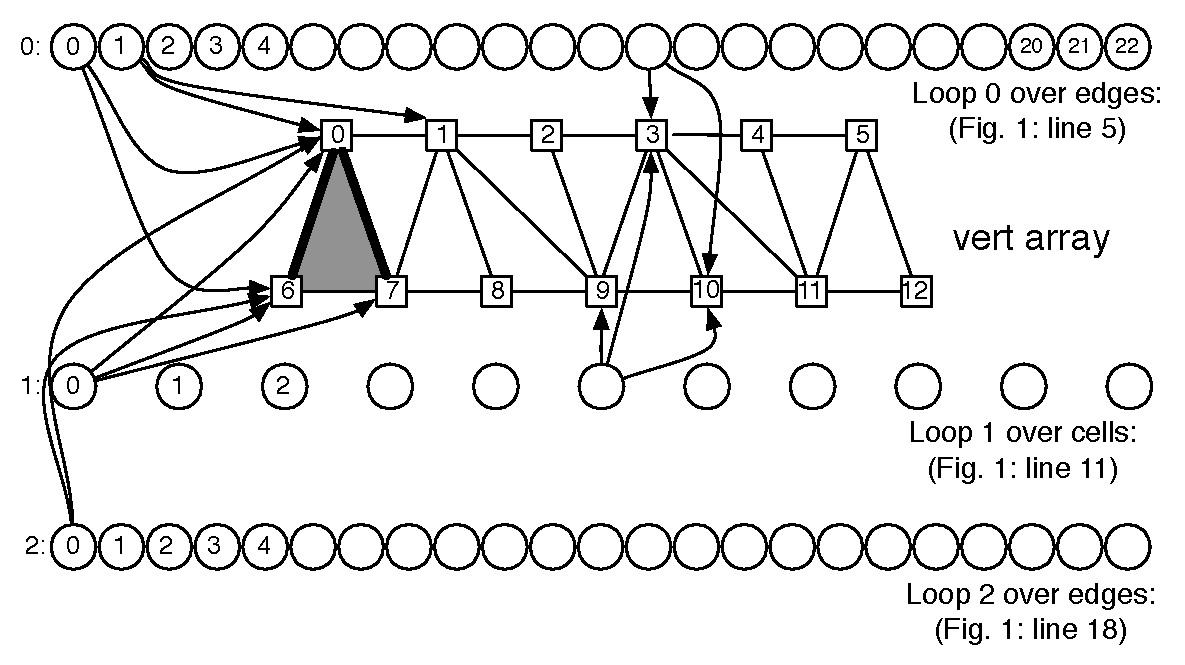
\includegraphics[scale=0.5]{sparsetiling/figures/tiling_example.pdf}
\caption{Visualization of a possible instance of the loop chain for the sequence of loops in Fig.~\ref{fig:op2-programexample}. The edge and cell loops use index arrays to indirectly access the data associated with the vertices in the mesh. Squares represent data associated with vertices in a mesh. Circles represent loop iterations. Note that iteration 0 in loop 0 visits the edge connecting vertices 0 and 6 and accesses the data associated with those vertices. Iteration 0 in loop 1 accesses all the vertices associated with the shaded triangular cell. Iteration 0 in loop 2 accesses vertices 0 and 6.}
\label{fig:loopchain}	
\end{figure}
~
%%%%%%%%%%%%%%%%%%%%%%%%%
%%%%%%%%%%%%%%%%%%%%%%%%%
\begin{figure}[t]
 \centering
		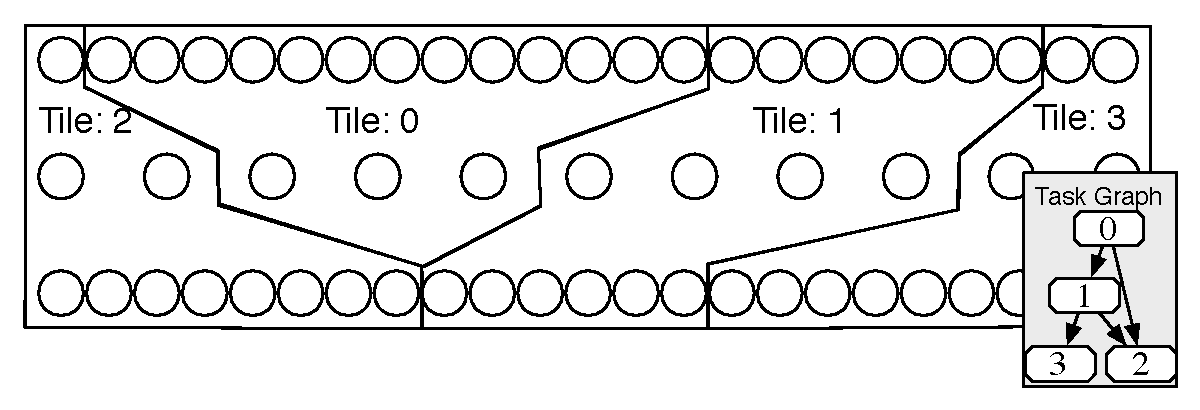
\includegraphics[scale=0.5]{sparsetiling/figures/tiling_example_tiled.pdf}
\caption{A sparse tiling for the loop chain in Fig.~\ref{fig:loopchain}.  The iterations
in the three loops have been placed into four tiles, which have been partially ordered
into a task graph.  The partial ordering arises from dependencies between iterations
in different tiles.}
\label{fig:fstOnOp2}	
\end{figure}
~
%%%%%%%%%%%%%%%%%%%%%%%%%

%  \item Contributions list:
% This is redundant and we can remove this when we are tight on space. -- Krieger
This paper's major contributions are as follows:
\begin{itemize}
\item A general full sparse tiling algorithm that applies to any sequence of loops that
  can be expressed using the loop chain abstraction.
%\item Examples illustrating the issues that arise when generalizing full sparse tiling and
%  explanations as to how the general algorithm deals with these issues.
% \item Properties in loop chains that can lead to simplifications in the 
% generalized full sparse tiling algorithm.
% %Specialization of the general full sparse tiling algorithm for use with the OP2 library
%  %for implementing unstructured-mesh applications.
%%  \item Adaptations to the general full sparse tiling algorithm to enable different parallelization
%%  targets: symmetric multiprocessors versus GPUs.  [distributed memory?]
  \item Performance evaluations of the full sparse tiling inspector/executor strategy 
  when applied to a Jacobi sparse matrix solver %, CoMD proxy application, 
  and the Airfoil computational fluid dynamics simulation.
\end{itemize}
%We also describe the issues that arise 
We identify a number of important issues arise when
 generalizing full sparse tiling, and we provide
explanations as to how the general algorithm deals with these issues.
Additionally, we describe how the key gFST algorithm concepts can
be adapted for use in the OP2 implementation context.
 
 % \item The outline paragraph.  Section 2 ...   Section 3 ... etc.
In Section~\ref{sec:loopchain}, we describe how data dependence relations can
be derived from the loop chain abstraction and indicate issues related to these
dependences that a general sparse tiling algorithm must handle.
These issues are addressed by the general full sparse tiling 
algorithm described in Section~\ref{sec:generalizedFST}.
Section~\ref{sec:OP2} describes adapting the OP2
parallelization algorithm to implement
generalized full sparse tiling.
Section~\ref{sec:evaluation} reports performance results,
Section~\ref{sec:relatedwork} covers work related to full sparse tiling, 
and Section~\ref{sec:conclusions} concludes the paper.

\section{Loop Chains for Generality}
\label{sec:loopchain}

% FIXME: MMS, need to fix broken citations that require reading my mind.

Sparse tiling techniques have been developed 
to improve the data locality within groups
    of iterations from different loops that share data and,
therefore, the performance of the overall computation.  {\em
  Inspector/executor strategies} implement sparse
tiling, where the executor is the transformed code with an added
tiling loop and the inspector is a new piece of code that visits index
arrays at runtime to determine how iterations can be legally and
profitably grouped into tiles.


%Sparse tiling is impleme
%are inspector/executor strategies that group
%subsets of iterations across loops into atomic tiles.  There is a partial
%ordering between these tiles, thus enabling parallelization when tiles
%do not share a dependence.  

%Previous approaches to sparse
%tiling have been specific to particular loop kernels.
%These approaches were based on inspecting
%the data dependencies between loops at runtime to perform
%a sparse tiling.  
This section reviews the loop chain abstraction,
describes how data dependences can be
derived from a loop chain, 
and presents issues that a general sparse tiling
algorithm of any kind must overcome.
The issues are that 
% MMS, I do NOT want these to be open parens.  They should be closed.
 (1) explicit inspection of the data dependencies
between loops to perform sparse tiling more generally is too 
computationally expensive (Section~\ref{sec:infeasible}),
 (2) when one or more of the loops being sparse 
tiled are performing
a reduction then there needs to be a partial ordering 
between tiles that perform
some reduction operation on the same data element (Section~\ref{sec:reduction}), 
and (3) when growing tiles to some loop $l$, 
it is important to consider
the dependencies of loop $l$ on all previous or all subsequent loops
(Section~\ref{sec:prevloops}). 
% FIXME might have to remove below for space.
Dependencies in these parallel loops are such that they can be from 
iteration in any loop $L_p$ to iterations in loop $L_q$ where $p<q$ in general.



%%%%%%%%%%%%%%%%%%%%%%%%%%%%%%%%%%%%%%%
\subsection{Data Dependence Analysis for Loop Chains}
\label{sec:loopchaindeps}
%%%%%%%%%%%%%%%%%%%%%%%%%%%%%%%%%%%%%%%

The previous sparse tiling approaches cited in Section~\ref{sec:intro} 
were specialized per benchmark.
In this paper we show how the loop chain programming abstraction~\citep{ST-KriegerHIPS2013}
can be used as a basis for generalized full sparse tiling.
As with all loop optimizations that reschedule the iterations in a sequence of loops, 
any sparse tiling must satisfy the data dependencies.
The loop chain abstraction provides enough information 
%to a compiler and/or
%run-time [FIXME: remove compiler?] system 
to compute all of the dependencies in a computation.
When the data accesses in the loop chain involve indirect memory accesses
like those that are the focus of this paper, then the runtime, or inspector,
can determine the data dependencies by querying the data access information 
contained in the loop chain abstraction. % [FIXME: not much clear to me].

% MMS: paraphrased our loop chain definition from the HIPS paper.
% FIXME: Krieger, the flow in this paragraph is in pain.
As described in Krieger et al.~\cite{ST-KriegerHIPS2013}, a loop chain consists
of the following:
%\\
%$~~~~~L$ a sequence of $N$ loops, $L_0, L_1, ..., L_{N-1}$.\\
%$~~~~~D$ a set of $M$ data spaces, $D_0, D_1, ..., D_m$.\\
%$~~~~~R_{L_l\rightarrow D_d}(\vec{i})$ and 
%$W_{L_l\rightarrow D_d}(\vec{i})$\\
\begin{itemize}
\item $L$ is a sequence of $N$ loops, $L_0, L_1, ..., L_{N-1}$.
\item $D$ is a set of disjoint $M$ data spaces, $D_0, D_1, ..., D_{M-1}$.
\item $R_{L_l\rightarrow D_d}(\vec{i})$ and $W_{L_l\rightarrow D_d}(\vec{i})$, 
where the $R$ and $W$ access relations are defined over for each data space $D_d \in D$
and indicate 
which data locations in data space $D_d$ an iteration $i \in L_l$
reads from and writes to respectively.
\end{itemize}

The assumption in a loop chain is that each loop is a {\em fully parallel
loop} or a {\em reduction loop}.  Here a reduction loop is more general
than a scalar reduction loop.  In a reduction loop  
each iteration of the loop does a read, an associative and commutative operation, and a write
to some element(s) in an array, and multiple iterations could read, modify, write the
same data element.


The access relations in the loop chain abstraction enable a
general derivation of the storage-related dependencies between loops in
a loop chain.  
%The assumptions within loop chains indicate that there are
%either no loop carried dependencies within a loop or only reduction
%dependences between iterations of a loop.
The storage related dependencies between loops can be described
as either flow (read after write), anti (write after read), or 
output (write after write) dependencies. % (see Fig.~\ref{fig:deps}).
%The identification of these dependencies is further discussed in section~\ref{sec:generalizedFST}.
Loop $L_x$ always comes before loop $L_y$ in the loop chain.  
The flow dependencies can be enumerated by considering pairs of points 
($\vec{i}$ and $\vec{j}$) in the iteration spaces of the two loops $L_x$ and $L_y$:
%$$ \{ (x,\vec{i}) \rightarrow (y,\vec{j}) | 
%     W_{L_x \rightarrow D_d}(x,\vec{i}) \bigcap   
%     R_{L_y \rightarrow D_d}(y,\vec{j}) \neq 0 \}.
%    $$
\[
	\{ \vec{i} \rightarrow \vec{j} \; | \; \vec{i} \in L_x \wedge \vec{j} \in L_y \wedge 
	W_{L_x\rightarrow D_d}(\vec{i}) \cap R_{L_y \rightarrow D_d}(\vec{j}) \ne \emptyset \}.
\]
Anti and output dependencies are defined as expected.



There are reduction dependencies between two or more iterations of the same
loop when those iterations read, modify with a commutative and associative operator,
and write to the same location(s).  
The reduction dependencies in loop $L_x$ are 
\[
	\{ \vec{i} \rightarrow \vec{j} \; | \; \vec{i} \in L_x \wedge \vec{j} \in L_x \wedge W_{L_x\rightarrow D_d}(\vec{i}) \cap W_{L_x \rightarrow D_d}(\vec{j}) \ne \emptyset \}.
\]
The reduction dependencies between two iterations within the
same loop indicates that those two iterations must be executed atomically
with respect to each other.
%indicate that
%a partial ordering between the involved iterations is needed.



%%%%%%%%%%%%%%%%%%%%%%%%%%%%%%%%%%%%%%%
\subsection{Data Dependence Inspection Issue}
\label{sec:infeasible}
%%%%%%%%%%%%%%%%%%%%%%%%%%%%%%%%%%%%%%%

With the computations that have been sparse tiled in the past
(Jacobi, Gauss-Seidel, moldyn, matrix powers kernel), inspecting the dependencies
between loops was implemented by traversing index arrays.
For example, in Jacobi, each iteration of a loop accesses a set
of neighbors.  
% FIXME(still?): Krieger need code example here? maybe from HIPS?
If the sparse matrix is stored in compressed sparse row format %~\cite{CSR},
then there is a compact list of neighbor identifiers.  By iterating over this list
the dependence relation is being inspected.  The dependence relation can be
	$\{ [i] \rightarrow [j] \; | \; j \in neighbors(i) \}$.
%or
%\[
%	\{ [i] \rightarrow [j] \; | \; i \in neighbors(j) \}.
%\]
The inspector can traverse the domain for the $i$ %or $j$ 
iterations
and determine data dependencies via
%by traversing
the neighbor set.

More generally, traversing data dependencies between loops might require more computation
than is preferred in an inspector, which after all must be amortized over multiple iterations of the loop chain.
For example, the data dependencies between the first edge loop and the 
cell loop for the running example in Fig.~\ref{fig:loopchain} are
\[
	\{ [ i ] \rightarrow [ j ] \; | \; edges2vertices(i,*)=cells2vertices(j,*) \},
\]
where $*$ indicates any of the index arrays into vertices for edges or cells.
Therefore if an edge and a cell share a vertex, then there is a dependence from the edge
iteration to the cell iteration.

Inspecting this relation requires a doubly-nested loop that iterates
over all edges and then for each edge all cells, $O(|E|  |C|)$, where
$|E|$ is the number of iterations in the edge loop and $|C|$ is the number
of iterations in the cell loop.
In Section~\ref{sec:generalizedFST}, the generalized full sparse tiling
algorithm performs tile growth in $O(|E| + |C|)$ instead of $O(|E|  |C|)$
by avoiding the explicit traversal of data dependences.

Existing inspector/executor techniques for sparse tiling avoid
explicitly enumerating data dependencies between loops by being specialized
for specific computations.  Wavefront parallelization techniques
for do across loops also avoid explicit enumeration of data dependencies
by tracking how iterations access data.
Sparse tiling techniques are different in that they aggregate iterations into tasks
and determine a task graph instead of determining level sets containing fine
grained parallelism.  We use a similar approach of tracking data accesses
to avoid explicit data dependence enumeration.



%%%%%%%%%%%%%%%%%%%%%%%%%%%%%%%%%%%%%%%
\subsection{Handling Reductions}
\label{sec:reduction}
%%%%%%%%%%%%%%%%%%%%%%%%%%%%%%%%%%%%%%%

Strout et al.~\cite{ST-StroutPLDI03} sparse tiled the moldyn computation
across three of its loops.  The loop over interactions between atoms
was a reduction loop.  Due to reduction dependencies and the resulting computation being performed
serially, there was no need to consider dependencies between tiles.

In general, reduction dependencies require that
tiles performing a reduction operation to the same data element
are given some arbitrary
partial order to avoid concurrent execution, which could lead to data races.
%between tiles that perform a reduction operation to
%the same data element are not executed concurrently. 
%Executing them concurrently would lead to data races.

%%%%%%%%%%%%%%%%%%%%%%%%%%%%%%%%%%%%%%%
\subsection{Dependencies from Non-Adjacent Loops}
\label{sec:prevloops}
%%%%%%%%%%%%%%%%%%%%%%%%%%%%%%%%%%%%%%%

Existing sparse tiling techniques only inspect 
dependencies between adjacent loops.  This was
because of symmetry between dependencies that caused the dependencies
between a loop and much earlier loops to be covered by the transitive closure
of dependence steps between intervening loops.  In general,
a loop could have a dependence, for example an anti dependence,
on a loop that is not directly adjacent.  The generalized full sparse tiling
algorithm handles this case.
%We see this for example in
%molecular dynamics code that have the first loop read from an array
%that is written to in the third loop. 
  
%%%%%%%%%%%%%%%%%%%%%%
\section{Generalized Full Sparse Tiling Algorithm}
\label{sec:generalizedFST}
%%%%%%%%%%%%%%%%%%%%%%
%To avoid realizing all of the formal data dependencies in the loop chain at runtime, 
To handle all the issues discussed in Section~\ref{sec:loopchain}, the generalized
full sparse tiling algorithm uses the data access relations provided by the
loop chain abstraction and a data structure we call $\Psi$ that tracks
all tiles that write to and read from each data item in each loop 
to produce a valid execution schedule.
Using the given data access relations and the $\Psi$ data structure, 
the generalized algorithm is able
to satisfy the ordering constraints in the loop chain due to
data dependencies.
%flow, reduction, and storage related dependencies. 

%
%%%%%%%%%%%%%%%%%%%%%%
\subsection{Algorithm Description}
\label{sec:algorithm}
%%%%%%%%%%%%%%%%%%%%%%
The generalized full sparse tiling algorithm takes a loop chain
%information about the series of loops to be tiled 
and assigns each iteration of the loops to a tile.
Along with the iteration-to-tile mapping, a task graph representing a partial ordering of the tiles is generated.
More precisely, the input to the algorithm is a loop chain ($LC$), 
the index of the loop chosen for seed partitioning ($s$), and the number of tiles ($T$).
Note that any loop can be selected for seed partitioning, but heuristically a loop in the middle
of the loop chain results in fewer dependencies between tiles.
The number of tiles is a tuning parameter used to balance data locality and parallelism.
The output is a function $\theta$ that maps each iteration of each loop in 
the chain to a tile and a task graph $G$ that captures the
partial ordering among the tiles due to data dependencies.

The general full sparse tiling method for loop chains consists of four phases:
\emph{initialization, backward tiling,} \emph{forward tiling}, and \emph{task graph creation}.  
Algorithm~\ref{algo:generalizedFST} shows the pseudo-code.

%%%%%%%%%%%%%%%%%%
\begin{algorithm}[t]
\caption{The Generalized Full Sparse Tiling Algorithm}
\label{algo:generalizedFST}
\textbf{GeneralizedFullSparseTile}\\
  \KwIn{Loop Chain $LC=(L,D,R,W)$, $s$, $T$}
  \KwOut{$\theta$, $G$}
  \KwData{$\Psi_*$}
%~~\\ 
// Initialize all fields of $\Psi$ to top or empty set \\
%\ForEach{$D_d \in D$}{
%\ForEach{$\vec{j} \in D_{d}$}{
%\ForEach{$l~s.t.~L_l~in~L_1~to~L_N$}{
%	$\Psi_{FR}(d,\vec{j},l)=\Psi_{LR}(d,\vec{j},l)= \top$\\
%	$\Psi_{FW}(d,\vec{j},l)=\Psi_{LW}(d,\vec{j},l)= \top$\\
%	$\Psi_{R}(d,\vec{j},l)=\Psi_{W}(d,\vec{j},l)= \emptyset$\\
%	}
%}
%}
%~~\\
// Initialize the tiling function $\theta$ values to $\top$ \\
%\ForEach{$l | L_l \in \{L_0,L_1...L_N\}$}{
%\ForEach{$\vec{i} \in L_l$}{
%$\theta(l, \vec{i}) = \top$
%}
%}
%~~\\
$\theta(L_{s},*) = PartitionSeedSpace(L_{s}, R, W, T) $\\
UpdateAccessTable($\Psi_*,s$)\\
%~~\\
//Tile the loop chain \\
\ForEach{$L_l $ in $ L_{s-1}~to~L_{0}$}{
BackwardTile($L,l, R, W, \theta, \Psi_*$))
UpdateAccessTable($\Psi_*,l$)
}
\ForEach{$L_l$ in $L_{s+1}~to~L_{N-1}$}{
ForwardTile($L,l, R, W, \theta, \Psi_*$)
UpdateAccessTable($\Psi_*,l$)
}
%\ForEach{$L_l $ in $ L_{1}~to~L_{N}$}{
%ForwardTile($L,l, R, W, \theta, \Psi_*$)
%}
%~~\\
//  Partial ordering of tiles\\
G = BuildTaskGraph($L$,$D$,$\Psi_*$,$T$)
%~~\\
%~~\\
\Return{$\theta,G$}
%~~\\
%~~\\
\end{algorithm}



\emph{Phase 1: Initialize internal data.}
Data dependency information is required during task graph creation.
Rather than tracking data dependencies directly, which may be 
prohibitively expensive, the algorithm maintains information pertaining to 
data reads and writes with respect to tiles.
The set of tiles in a particular loop~($l$) that read a particular data item~($\vec{v}$) in 
data space~($d$) is denoted as $\Psi_R(d,\vec{v},l)$.
The tiles that write are tracked in a similar set $\Psi_W(d,\vec{v},l)$.

Additionally, tile data access information is used during backward and forward tiling.
Associated with each of the $\Psi_R$ and $\Psi_W$ sets are single values that record the 
first and last tiles that access
a specific data element.
$\Psi_{LR}(d,\vec{v},l)$ is the last read performed on the $v^{th}$ data element of 
the data space $D_d$ from loop $L_l$.
Replacing the subscripts with FR, FW, and LW correspond to the first read, 
first write and last write respectively.
The initialization phase initializes all the tile assignments to top ($\top$) and sets
all of the data access information in $\Psi$ to empty set or top as appropriate.

The initialization phase also includes a preliminary partitioning of the seed loop's iteration space, $L_s$.
Partitioning the seed loop involves assigning each iteration of the seed loop to a tile. 
%The partitioning is performed using a graph partitioner called ParCubed \cite{KriegerLCPC2012}.
$UpdateAccessTable$ updates the values in all internal state data sets ($\Psi_*$) with respect to the 
seed partitioning.  Specifically, since there is a tile assignment for all the iterations in the
seed loop, it will be possible to determine the set of tiles that read and write to each data element
accessed in that seed loop.

For example, Fig.~\ref{fig:tiling_psi_time} shows a portion of the $\Psi$ data structure
for the loop chain example in Fig.~\ref{fig:loopchain}.  
In this example, the seed loop is chosen as loop 1.
This is the loop over cells (a cell is a triangle here).
In this example we follow the creation of tile 2.
After the seed partitioning, iterations 0 and 1 in loop 1 are in tile 2, 
$\Theta(1,0)=2$ and $\Theta(1,1)=2$.
The $\Psi$ data structure
contains tile access information for each data element (i.e., vertices in the mesh)
at each loop in the computation (i.e., note three columns for each vertex, one for each of the
three loops).  The left side of Fig.~\ref{fig:tiling_psi_time} shows the initial write
sets for part of the {\tt vert} data structure.  The first two cells have been put into
tile 2 in the seed partition loop.  The vertices adjacent to these two cells have
a 2 in the center column to illustrate that the tile 2 is in the sets $\Psi_W(vert,0,1)$ and $\Psi_W(vert,1,1)$.
The zeros in the middle columns of the $\Psi$ table are for vertices adjacent to
cells that are in tile 0.


\begin{figure}[t]
\centering
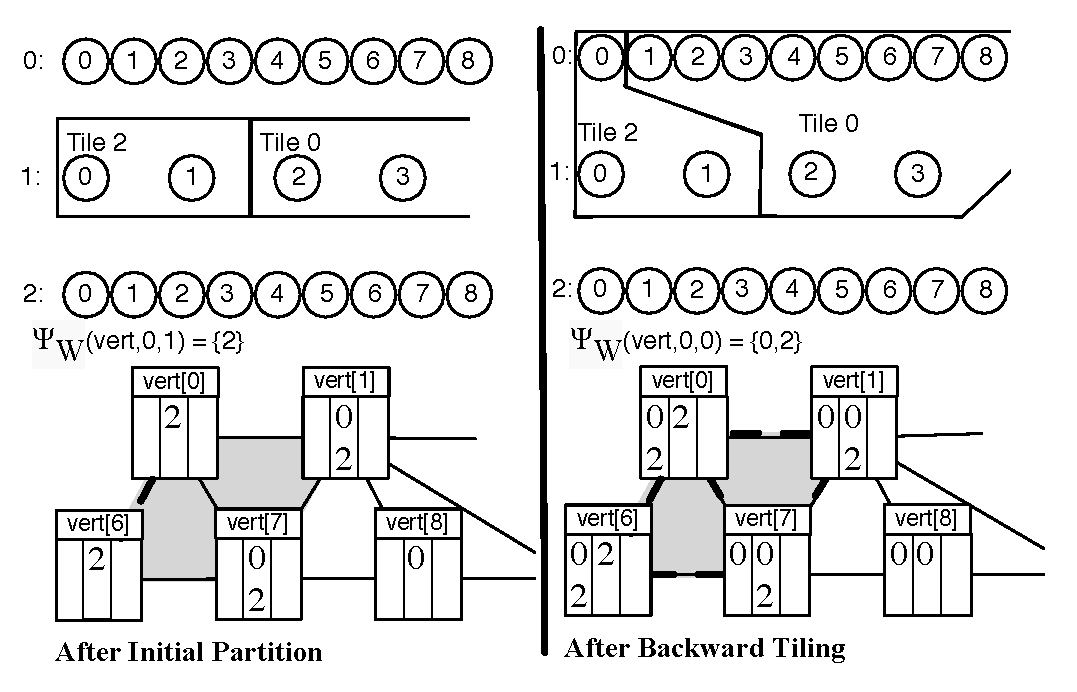
\includegraphics[width=\columnwidth]{sparsetiling/figures/psi_timestep.pdf}
\caption{This figure illustrates part of the evolution of the $\Psi_W$ data structure for the 
loop chain example in Fig.~\ref{fig:loopchain}.  After the initial seed partitioning
of loop 1, which iterates over cells, the middle columns (loop 1) associated with each vertex
includes the set of tiles for cells that are adjacent to the vertex.  After backward tiling,
the $\Psi_W$ data structure is updated to include the tile numbers for all the edges
that access a vertex in loop 1.  Only one edge is in tile 2 in loop 0, so all vertices shown
are written to by edges in Tile 0. }
\label{fig:tiling_psi_time}	
\end{figure}


\begin{algorithm}[t]
\caption{The Backward Tiling Algorithm}
\label{algo:backwardTiling}
\textbf{BackwardTile}\\
  \KwIn{$LC,l, \Psi_*$} 
  \KwOut{$\theta$}%, \Psi_*$}%.\{firstread, lastread, firstwrite, lastwrite, reads, writes\}}
%~~\\
Define: MIN($\top$,X) = X.\\
\ForEach{$\vec{i} \in L_{l}$}{
// all datasets \\
\ForEach{$d \in D$}{
// all data elements read by this iteration \\
 \ForEach{$\vec{v} \in R_{L_l\rightarrow D_d}(\vec{i})$}{
 // each later loop's access tables\\
%	\ForEach{$L_{k}\in\{L_{l+1}~to~L_{N-1}\}$}{
%% MMS, 10/14/13, only going to s because later loops don't have Psi values yet.
	\ForEach{$L_{k}\in\{L_{l+1}~to~L_{s}\}$}{ 
	// anti dependence\\
	$\theta(l, \vec{i}) = MIN( \theta(l,\vec{i}), \Psi_{FW}(d,\vec{v},k)$) \\
}
}
// all data elements written by this iteration \\
 \ForEach{$\vec{v} \in W_{L_l\rightarrow D_d}(\vec{i})$}{
%	\ForEach{$L_{k}\in\{L_{l+1}~to~L_{N-1}\}$}{ 
%% MMS, 10/14/13, only going to s because later loops don't have Psi values yet.
	\ForEach{$L_{k}\in\{L_{l+1}~to~L_{s}\}$}{ 
	// output dependence\\
	$\theta(l, \vec{i}) = MIN( \theta(l,\vec{i}), \Psi_{FW}(d,\vec{v},k)$) \\
	// flow dependence\\
	$\theta(l, \vec{i}) = MIN( \theta(l,\vec{i}), \Psi_{FR}(d,\vec{v},k)$) \\
}
}
} %foreach
} % foreach

%~~\\
%~~\\
\end{algorithm}


\emph{Phase 2: Backward Tiling.}
The result of tiling is that each iteration in the loop chain is assigned to a tile. % or task.
Backward tiling (see Algorithm~\ref{algo:backwardTiling}) starts with the iterations in
the seed partitions and grows tiles to earlier loops ensuring that the data dependencies are
satisfied.
% is performed by assigning 
%iterations to tiles based on their data accesses, 
%Backward tiling starts with the loop directly before the seed loop and stepping backwards to the first.
%The three types of data dependencies are accounted for: flow, anti, and output.
Each iteration in the loop being tiled is assigned to either the existing tile assignment 
or $\Psi_{FW}(d,\vec{v},l)$ or $\Psi_{FR}(d,\vec{v},l)$, depending on which occurs first (the result of $MIN$).

Consider the running example in Fig.~\ref{fig:tiling_psi_time}. 
Backward tiling in this example only occurs on loop 0.
Iteration 0 in loop 0 starts with a tile value of top, $\Theta(0,0) = \top$.
Iteration 0 in loop 0 does a reduction operation on two vertices 
(0 and 6, the edge is represented as a bold, dashed line)
and we have 
%$\Psi_W(vert,0,1) = \Psi_W(vert,6,1) = \{2\}$ 
$\Psi_{FW}(vert,0,1) = 2$ and $\Psi_{FW}(vert,6,1) = 2$.
Therefore, iteration 0 of loop 0 is assigned to tile 2, $\Theta(0,0) = 2$.
As another example, iteration 1 of loop 0 accesses the vertices 0 and 1, and
$\Theta(0,1) = \top$, 
$\Psi_{FW}(vert,0,1) =  2$, and $\Psi_{FW}(vert,1,1) = 0$.
% FIXME: check this
$MIN(\Theta(0,1),\Psi_{FW}(vert,0,1),\Psi_{FW}(vert,1,1)$  is 0 and therefore iteration 1 
in loop 0 is assigned to tile 0, $\Theta(0,1)=0$.
Intuitively any time an earlier loop iteration will be writing to a data item that an iteration in
a later loop accesses, then the earlier loop iteration needs to be in the same or
earlier tile.

Once the tile assignments are chosen, $\Psi_*$ is updated to reflect the changes.
These values are reflected in the first column of each vertex in Fig. \ref{fig:tiling_psi_time}.


\emph{Phase 3: Forward Tiling.}
In this phase, loops after the 
seed space are tiled. This process starts with the iteration space immediately 
following the seed loop and proceeds forward, loop by loop, until 
reaching the last loop in the chain. The forward tiling algorithm uses $MAX$ where
the backward tiling algorithm uses $MIN$. It exploits the last read and write information
to ensure data dependencies are satisfied.


%%%%%%%%%%%%%%
\begin{algorithm}[t]
\caption{The task graph %, which encodes the partial ordering between tiles due
%to data dependencies, 
is determined by inspecting all tiles
that read and write to each data element.}
\label{algo:buildTaskGraph}
\textbf{BuildTaskGraph}\\
  \KwIn{$L,D,\Psi_*,T$}
  \KwOut{$G=(V,E)$}

$E=\emptyset, V = \{ 0, 1, \cdots, T-1\}$ // Each tile is task \\

%	For each data item d
\ForEach{$d~s.t.~D_d~in~D_0~to~D_{M-1}$}{
%		For each loop l
\ForEach{$l~s.t.~L_l~in~L_0~to~L_{N-1}$}{
\ForEach{$\vec{v} \in D_d$}{
// Reductions\\
$E = E \cup \{[s] \rightarrow [t] \; | \; s \in \Psi_W(d,\vec{v},l) \wedge$\\
$~~~~~ t \in \Psi_W(d,\vec{j},l) \wedge s<t\}$\\
%put an edge from a lower numbered tile to higher numbered tiles for all pairs of tiles that write to a particular data item
// Flow dependencies\\
\ForEach{$k~s.t.~L_k~in~L_l~to~L_0~until~\Psi_{LW}(d,\vec{v},k) \ne \top$}{
%(flow) put an edge starting at AT(d, $L_k$).lastwrite and ending at each tile in AT(d, $L_j$).reads such that k<j.
%\ForEach{$T_j \in AT(d, L_k).reads \wedge k<j$}{
%$E \gets (AT(d,L_k).lastwrite,T_j)$
%}
$E = E \cup \{[s] \rightarrow [t] \; | \; s=\Psi_{LW}(d,\vec{v},k) \wedge $\\
$~~~~~ t \in \Psi_R(d,\vec{j},l) \wedge  s<t\}$\\
}
// Anti dependencies\\
\ForEach{$k~s.t.~L_k~in~L_l~to~L_{N-1}~until~\Psi_{FW}(d,\vec{j},k) \ne \top$}{
$E = E \cup \{[s] \rightarrow [t] \; | \; s \in \Psi_{R}(d,\vec{v},l) \wedge $\\
$~~~~~ t=\Psi_{FW}(d,\vec{v},k) \wedge  s<t\}$\\
}
%(anti) put an edge starting at each tile in AT(d,$L_k$).reads to d to the firstwrite to this data item in the earliest subsequent loop AT(d, $L_j$).firstwrite such that k<j for the first j that has a write to this data item.
// Output dependencies \\
			%(output) put an edge starting at AT(d, $L_k$).lastwrite and ending at the first j>k where AT(d, $L_j$).firstwrite != AT(d, $L_k$).lastwrite
\ForEach{$k~s.t.~L_k~in~L_l~to~L_{N-1}~until~\Psi_{FW}(d,\vec{v},k) \ne \top$}{
$E = E \cup \{[s] \rightarrow [t] \; | \; s=\Psi_{LW}(d,\vec{v},l)  \wedge$\\
$~~~~~ t=\Psi_{FW}(d,\vec{v},k) \wedge s<t \} $\\
}
}
}
}
\end{algorithm}
% FIXME: Cathie (DONE) , please fix the formatting in the above.  I modified the constraints like we discussed.
% FIXME: Cathie -> MMS the inner loops over k are expressed a little weird.
%%%%%%%%%%%%%%


\emph{Phase 4: Task Graph Creation.} The edges in the task graph 
represent the data dependencies that occur between iterations in different tiles
(for example see Fig.~\ref{fig:fstOnOp2}). 
%exposes 
%the data dependency information implicitly stored in the $\Psi_*$ sets.
The four steps of the task graph creation, as shown in Algorithm~\ref{algo:buildTaskGraph}, correspond to the four types of dependencies between tiles. 
%Edges representing reduction dependencies are discovered by taking the 
%cartesian product of the set of tiles that write to a specific data element within a specific loop with itself. 
To avoid cycles in the task graph, the source tile of an edge should always be
numbered lower than the target tile for the edge.
%an edge has to start and end at 
%different tiles and its direction has to be from a lower to a higher tile.

%% MMS: can we get away without having this?
Reduction dependencies are detected when a single entry in the
$\Psi_W$ table includes multiple tiles, thus indicating that multiple
tiles are writing to a single vertex in the same reduction loop.
A partial ordering from the lower to higher numbered tiles
is placed in the task graph to avoid data races.
Edges representing flow dependencies are created by connecting all 
tiles that read a specific data element within a given loop to the tile that 
has most recently written to that data element in a previous loop. 
Anti-dependence edges are similar, but connect all of the tiles that 
read a given element in a given loop to the first tile in a subsequent 
loop that writes to the tile.
Output dependences are found by connecting the last write of a data 
element to the first write of the same element in subsequent loops.

The generalized full sparse tiling algorithm maps each iteration in the loop chain
to a tile with the tile mapping function $\theta$ and generates a partial
ordering between the tiles in the form of a task graph.
One possible execution model is to then execute each tile/task
serially (loops executed in the original loop sequence within each tile)
and to execute tiles/tasks that do not share a partial ordering in parallel.


%%%%%%%%%%%%%%%%%%%%%%
\subsection{Algorithm Complexity and Correctness}
\label{sec:correctness}
%%%%%%%%%%%%%%%%%%%%%%

The backward (and forward) tiling algorithms traverse
all iteration and data index pairs in the read $R_{L \rightarrow D}$
and write $W_{L \rightarrow D}$ relations.
For each such pair, the impact of all previous loops in the loop chain
on the data item in question are queried in the $\Psi$ data structure (line 10
of the Backward Tiling algorithm).
Therefore the complexity is $O(NMP)$ complexity, where $N$ is the total 
number of iterations in the loop chain,
$M$ is the average number of data accesses per iteration, and
$P$ is the number
of loops in the loop chain.
Note that $NM$ is the number of pairs in the read $R_{L \rightarrow D}$
and write $W_{L \rightarrow D}$ relations.
We
avoid $O(N^2)$ behavior such as the $O(|E| |C|)$ from Section~\ref{sec:infeasible}
that would be needed if all data dependencies between iterations were explicitly determined.

% all of the iterations in
%a loop chain and all of the data accesses in a loop chain.  As such we
%avoid $O(nm)$ behavior where $n$ and $m$ are the number
%of iterations in any two loops.  Line 10 of the Backward Tiling algorithm
%does traverse all of the loops after the loop for the current iteration.
%This does result in $O(pq)$ complexity, where $p$ is the number
%of loops in the loop chain and $q$ is the total number of iterations in
%the loop chain.  Each iteration maintains inform
%however the number of loops $p$ is small.
We do need to explicitly determine dependencies between tasks to specify the
task graph.
The task graph construction algorithm has a worst case complexity
of $O(T^2)$, where $T$ is the number of tiles, because
all of the tiles
could read or write to a particular data element.
However, if that were the case, then the problem is not sparse enough for full sparse tiling
to be effective.
% and that would cause $O(T^2)$,
%where $T$ is the number of tiles,
%work to enumerate the partial orderings due to reductions.


Any schedule for iterations in a loop chain is correct if
the schedule satisfies the partial ordering between iterations
in the loop chain dictated by the data dependencies
detailed in Section~\ref{sec:loopchaindeps}.
The full sparse tiling algorithm indirectly satisfies these 
data dependencies without actually having to explicitly construct
the data dependencies at runtime.
%We provide the outline of a proof for why this is the case.
The full proof is omitted due to space.


%%%%%%%%%%%%%%%%%%%%%%
%\section{Sparse Tiling in OP2}
\section{OP2 implementation of gFST}
\label{sec:OP2}

OP2\footnote{OP2 denotes that this is the second generation of the 
OPlus library, or Oxford Parallel Library.} is a library for implementing 
applications that solve partial differential equations over unstructured 
meshes. For example, OP2 is employed in the Hydra CFD application, 
used at Rolls Royce for the simulation of next-generation components 
of jet engines, and in Volna~\citep{ST-volna}, a CFD application for the 
modelling of tsunami waves. These applications are composed of a 
large number of parallel or reduction loops (hundreds in Hydra, tens 
in Volna).  This section describes how we adapted the current
OP2 parallelization algorithm to implement generalized full sparse tiling
for OP2 programs.  Inclusion of the calls to the OP2 gFST inspector
and introduction of tile loops into the executor code is done manually.
The goal is to assess the performance of gFST in the context
of a mature code base like OP2, before incorporating
this optimization into the OP2 compiler.
%This is one of the required steps towards making this optimization
%part of the OP2 compiler.

%The aim is to provide a proof of concept GFST library 
%implementation for assessing performance in the context of a 
%mature code base. This is one of the required steps towards making 
%the algorithm part of the OP2 compiler. 


%%%%%%%%%%%%%%%%%%%%%%
\subsection{Loop chains in the OP2 Library}
\label{sec:OP2overview}


OP2 offers abstractions for modeling an unstructured mesh in terms 
of sets, datasets and mappings between sets. OP2 programs are expressed as 
sequences of parallel loops, each loop applying a user-programmed 
function, or ``kernel'', to every element in the iteration set. For each 
set element, datasets are accessed through 
maps. For example, the parallel loops in the program in Fig.~\ref{fig:op2-programexample} 
iterate over sets of mesh elements ({\tt edges}) and access 
datasets ({\tt vert}) via mappings, which can be indirect 
({\tt edges2vertices}) or direct ({\tt op\_id}).

In OP2, access modes are used to indicate how datasets are being 
accessed: (1) {\tt OP\_READ} - the dataset is only read, (2) {\tt OP\_WRITE} - 
the dataset is written to, (3) {\tt OP\_INC} - an increment for each value of 
that dataset is computed without reading the actual value of the dataset.
An access descriptor (op\_arg\_dat) contains: a dataset, a mapping and an access mode.
Each parallel loop contains an access descriptor for each dataset used by the kernel. This
information captures the loop chain abstraction in OP2. 



\subsection{Specializing gFST for OP2 Loop Chains}
\label{sec:OP2gFSTalg}

The standard OP2 OpenMP parallelization is done on a per loop basis
and is achieved by block partitioning the iteration set (e.g. cells, edges). In the OP2 gFST inspector, instead, partitioning occurs only once and is performed on the mesh vertices. These partitions are 
grown to tiles in the backward and forward tiling operations. In both cases, 
serialization of iterations incrementing the same 
value (i.e., reduction dependencies) is enforced by giving a color to 
partitions and allowing only same-colored partitions to execute in 
parallel, with iterations inside a partition being executed sequentially. 

The OP2 gFST inspector extends this technique by coloring partitions 
to respect tile-to-tile dependencies exposed  by the forward and backward tiling operations. 
The inspector builds a seed partition graph (SPG) with each 
node of the SPG being a partition of vertices. 
Edges are inserted in the SPG
based on the $K$-reachability relation between partitions: if two vertices in
separate partitions are within $K$ edges or cells of each other then 
their corresponding partition nodes in the SPG will be connected. 
Building the SPG costs $O(TN(B^K))$, where $T$ is the number of tiles, $N$ 
is the number of vertices on the border of a partition, 
$B$ is the average out degree for vertices in the mesh, and $K$ is how
many edges the depth-first search visit traverses from each border vertex.
In our examples $B$ is 3 or 4, $K$ is the number of loops in the loop chain and tends
to be small, and $N$ is around 40.
The SPG is then 
colored %using the standard OP2 algorithm 
to prevent same-colored tiles
from sharing a dependence. 
%from becoming adjacent as tiles grow. For each loop we tile over, tiles can 
%shrink or expand. The value of $K$ depends on the number of loops in the 
%chain and assumes the worst case in which tiles always expand. This avoids 
%any possible race conditions due to parallel execution.

The gFST algorithm tracks all the tiles that read from and 
write to a particular data item in \emph{each} loop. This information, stored in the 
$\Psi_*$ data structure, is used to determine a partial order of tile execution 
due to data dependencies. %(see Fig.~\ref{fig:deps}) 
%and, therefore, impacts the cost of tiling. 
The OP2 gFST simplifies dependency tracking by exploiting the fact that vertices are accessible 
by all iteration set via mappings. 
Instead of storing all the tiles that read
and write to a particular vertex per loop, it is only necessary to track the first
tile that reads or increments a vertex while doing backward tiling and the last tile that
reads or increments a vertex while doing forward tiling.
Specifically the complexity of the OP2 gFST tile growth
is $O(NM)$ instead of $O(NMP)$, where 
where $N$ is the total 
number of iterations in the loop chain,
$M$ is the average number of data accesses per iteration, and
$P$ is the number
of loops in the loop chain; the loop at Line 4 in Algorithm 3 is unnecessary.


Adapting the existing OP2 parallelization algorithm to perform gFST highlights the most crucial aspects of the
algorithm while illustrating that these features can be specialized for
particular implementation contexts. The most crucial features are 
(1) there needs to be some mechanism for providing a seed partitioning,
whether on an iteration space or a data space that all iteration spaces access
directly or indirectly, (2) flow, anti, and output dependencies need to be respected 
during backward and forward tile growth to maintain tile atomicity,
(3) flow, anti, output and reduction dependencies between tiles need to be partially ordered
to avoid data races.




%%%%%%%%%%%%%%%%%%%%%%%%%%%%%%%%%%%%%%%%
%%%%%%%%%%%%%%%%%%%%%%%%%%%%%%%%%%%%%%%%
\section{Evaluation of Generalized Sparse Tiling}
\label{sec:evaluation}
% "In order to" should almost always just be replaced with "To" in formal writing.
%In order to 
To evaluate the performance improvements achieved by full sparse tiling, we conducted several experiments. 
%For the experiments using gFST, 
In all the experiments, the optimal tile size (i.e. the one leading to the best execution time) was determined empirically, for each combination of machine and application. Our objective is to explore 
the impact of gFST on %serial and parallel 
performance, and to characterize the circumstances where the approach is profitable.
% FIXME: we need more of an overview here.


\subsection{The Sparse Jacobi Benchmark}
\label{sec:gfst-evaluation}

%%%%%%%%%%
\begin{figure*}[t]
\centerline{
    \subfigure[]{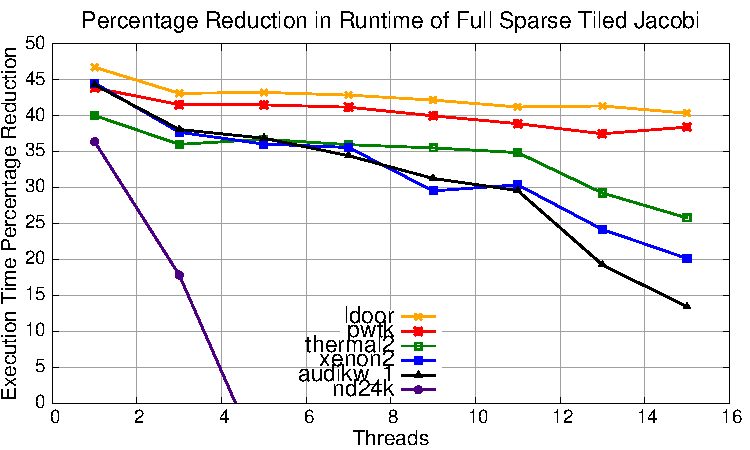
\includegraphics[scale=0.62]{sparsetiling/figures/JacobiImprovement.pdf}\label{fig:jacobiImprovement}}
    \subfigure[]{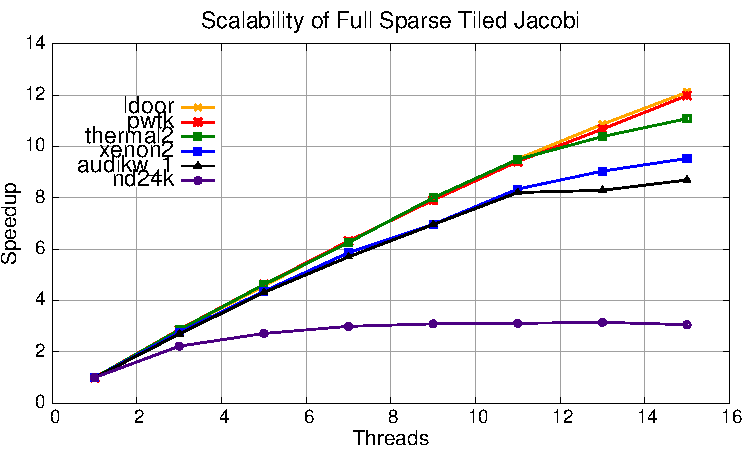
\includegraphics[scale=0.62]{sparsetiling/figures/JacobiSpeedup.pdf}\label{fig:jacobiSpeedup}}
}
\caption{The Jacobi solver's loop chain performance in terms of percentage reduction over the simple blocked parallel version, and speedup over the sequential full sparse tiled versions. Results for 6 different sparse matrices are shown. The nd24k line goes off the chart, reaching -152 percentage reduction at 15 cores; full sparse tiling does not always result in better performance.}
\label{fig:jacobi}
\end{figure*}
%%%%%%%%%%

The first experiment was the full sparse tiling of a Jacobi sparse matrix solver. Given a sparse matrix $A$,
and a vector $\vec{f}$, related by $A\vec{u}=\vec{f}$, each iteration of the sparse Jacobi method produces
an approximation to the unknown vector $\vec{u}$. In our experiments, the Jacobi convergence 
iteration loop is unrolled by a factor of two and the resulting two loops are chained together 
(1000 iterations of the loop chain
was executed).
Using a ping-pong strategy, each loop reads from one copy of the $\vec{u}$ vector 
and writes to the other copy. This experiment was run on an Intel Westmere 
(dual-socket 8-core Intel Xeon E7-4830 2.13 GHz, 24MB shared L3 cache per socket).
The code was compiled using {\tt gcc-4.7.0} with options {\tt -O3 -fopenmp} and OpenMP tasks were used
to execute the task graph. 
%Two thousand convergence iterations were performed for each matrix by executing the loop chain 1000 times. 

The Jacobi recurrence equation includes a sparse matrix vector multiplication and is representative of a broad class of sparse linear algebra applications. It is also an effective testbed because different data dependency patterns can be examined simply by using different input matrices. In these experiments, a set of 6 input matrices, drawn from the University of Florida Sparse Matrix Collection~\citep{ST-MatrixMarket}, was used. The matrices were selected so that they would vary in overall data footprint, from 45 MB to 892 MB, and in percentage of non-zeros, from very sparse at 0.0006\% to 
%significantly 
much more dense at 0.5539\% non-zeros. % values.

Figure~\ref{fig:jacobi} (left) shows the execution time reduction achieved by full sparse tiling the Jacobi solver  compared with the execution time of a simple blocked parallel version using OpenMP \texttt{parallel for} directives on the unrolled loops. The execution time reduction varied from 13\% to 47\% with the exception of the nd24k matrix, which showed as much as a 1.52x slowdown when full sparse tiled. This matrix is highly connected and yields a task graph that has limited parallelism. The greater parallelism available under a blocked approach provides more benefit in this case than the performance improvements due to improved locality from full sparse tiling.
%and typically decreased as threads were added. We believe that this reduction is also related to the parallelism available in the task graph and are investigating methods to mitigate its impact.

These execution times do not include the inspection time necessary to full sparse tile the loop chain. To break even when this cost is considered, the inspector time must be amortized over between 1000 and 3000 iterations of the executor, depending on the specific matrix being solved. As the inspector code matures and becomes more efficient, this cost will diminish.

In Figure~\ref{fig:jacobi} (right),  the scalability of the full sparse tiled Jacobi solver is shown. In general, speedups of between 8 and 12 times over the single-threaded performance were observed when using 15 threads. A clear outlier is again the nd24k matrix that did not scale past 3.2 times the single thread performance. The high degree of connectivity present in this matrix limited the parallelism available in the task graph, which in turn limited the scalability.

\subsection{OP2 Airfoil Benchmark}

\begin{figure*}[t]
\centerline{
    \subfigure[]{\label{fig:airfoil-t-sb}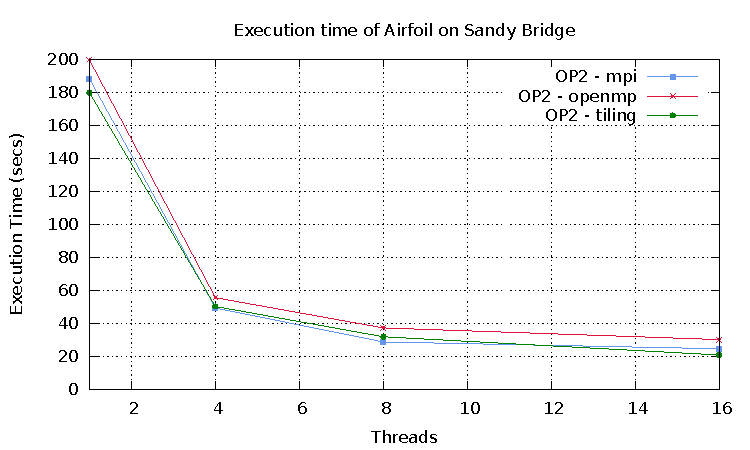
\includegraphics[scale=0.62]{sparsetiling/figures/op2-new-res/sb/time-intel-sandyb.pdf}}
    \subfigure[]{\label{fig:airfoil-t-w}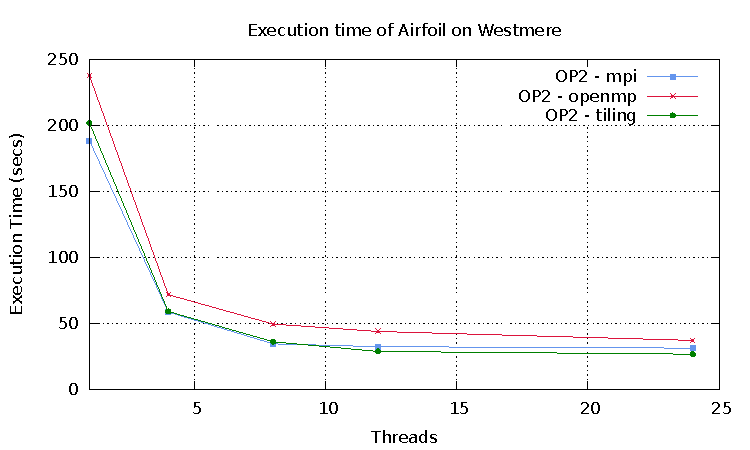
\includegraphics[scale=0.62]{sparsetiling/figures/op2-new-res/west/time-intel-westmere.pdf}}
}
\centerline{
    \subfigure[]{\label{fig:airfoil-s-sb}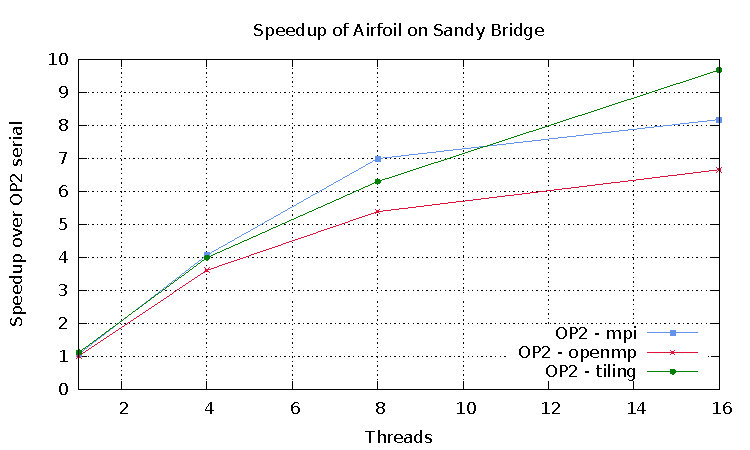
\includegraphics[scale=0.62]{sparsetiling/figures/op2-new-res/sb/speedup-intel-sandyb.pdf}}
    \subfigure[]{\label{fig:airfoil-s-w}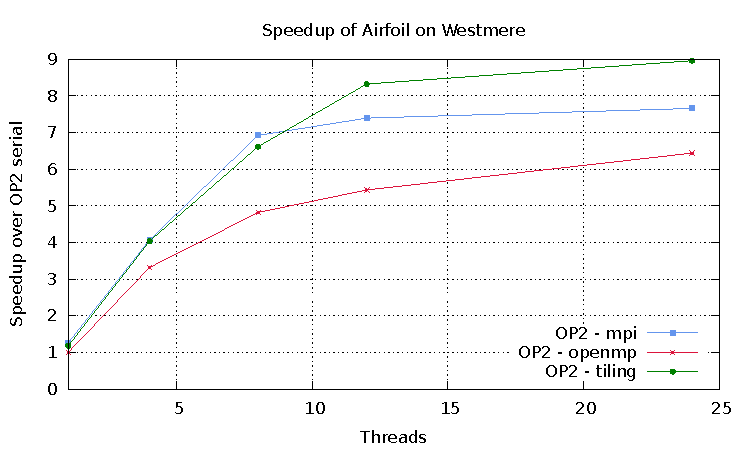
\includegraphics[scale=0.62]{sparsetiling/figures/op2-new-res/west/speedup-intel-westmere.pdf}}
}
       \caption{The Airfoil's loop chain performance in terms of execution time (in seconds) and speedup relative to the best sequential execution time for Sandy Bridge(a,c) and Westmere(b,d). The speedup is evaluated with respect to the $omp$ version with one thread (i.e. the slowest sequential back-end).}
\label{fig:sandy}
\end{figure*}


The OP2 adaptation of the generalized sparse tiling technique was evaluated in a representative unstructured mesh application called Airfoil~\citep{ST-AIRFOIL}. Three implementations of Airfoil, namely $omp$, $mpi$ and $tiled$, were compared on two shared-memory machines, an Intel Westmere (dual-socket 6-core Intel Xeon X5650 2.66 GHz, 12MB of shared L3 cache per socket) and a more recent Intel Sandy Bridge (dual-socket 8-core Intel Xeon E5-2680 2.00Ghz, 20MB of shared L3 cache per socket). The code was compiled using the Intel \texttt{icc 2013} compiler with optimizations enabled (\texttt{-O3}, \texttt{-xSSE4.2/-xAVX}).

The OP2 Airfoil application consists of a main time loop with 2000 iterations. This loop contains a sequence of four parallel loops that carry out the computation. In this sequence, the first two loops, called $adt$-$calc$ and $res$-$calc$, constitute the bulk of the computation. $Adt$-$calc$ iterates over cells, reads from adjacent vertices and write to a local dataset, whereas $res$-$calc$ iterates over edges and exploits indirect mappings to vertices and cells for incrementing indirect datasets associated to cells. These loops share datasets associated with cells and vertices. Datasets are composed of doubles.
%-precision floating-point values.

In the $omp$ and $mpi$ implementations of Airfoil, the OpenMP and the MPI back-ends of OP2, were used. The effectiveness of these parallelization schemes has been demonstrated in~\cite{op2-main}. The OP2 OpenMP back-end has been intuitively described in Section~\ref{sec:OP2}. The $tiled$ implementation exploits the OP2 gFST library for tiling a loop chain composed of 6 loops: the time loop was unrolled by a factor of two so as to tile over $adt$-$calc$ and $res$-$calc$ twice. The OP2 gFST library uses $METIS$~\citep{METIS} for computing a seed partitioning
of the mesh vertices.
% set of vertices between the two loops.

Figure~\ref{fig:sandy} shows the scalability and runtime reduction realized by full sparse tiling the loop chain on the Westmere and Sandy Bridge machines. The input unstructured mesh was composed of 1.5 million edges. It is worth noticing that both the $omp$ and $tiled$ versions suffer from the well-known NUMA effect as threads are always equally spread across the two sockets. It is left as further work extending gFST algorithms to work around this issue. Nevertheless, compared to $mpi$, the $tiled$ version exhibits a peak runtime reduction of 15\% on the Westmere and of 16\% on the Sandy Bridge.  %Figures~\ref{fig:airfoil-s-mc} and~\ref{fig:airfoil-t-mc} illustrate the results of analogous experiments on the Intel Manycore machine on which a runtime reductuon of 50\% was observed. A first difference from the experiments carried out on Sandy Bridge and Westmere is that, due to a better usage of the memory bandwidth, the $staged$ version runs faster than $plain$. The full sparse $tiled$ version, however, not only outperforms $staged$ in terms of execution time, but also improves the scalability up to high parallelism degrees.  

%Compared to $mpi$, which runs faster than $omp$ due to a better exploitation of the ,.
%We also note that as the number of threads employed increases, full sparse tiling shows an increasing benefit

% IMPACT INSPECTOR:
Results shown for $tiled$ do not include the overhead of the inspector. By also including the inspector cost, the aforementioned improvements over $mpi$ reduce to roughly 10\% on both platforms. However, as the time-marching loop in real-world OP2 applications tends to be larger than in Airfoil, we expect the overhead of the inspector to be, in general, smaller. In addition, we believe the current implementation of the gFST inspector is amenable to several optimisations. 


%%%%%%%%%%%%%%%%%%%%%%%%%%%%%%%%%%%%%%%%
\subsection{Discussion of the Performance Results}

The performance results presented here for Jacobi and Airfoil support 
previous work demonstrating the benefits of full sparse 
tiling~\citep{ST-StroutIJHPCA,ST-StroutPLDI03,ST-commAvoidingSparse2009}.
Extending this approach by grouping iteration that share data across 
loops into tiles improves performance due to improved data locality. 
On multicore machines this avoids memory bandwidth saturation while scaling.

Insufficient parallelism in the task graph can limit the performance improvements. 
This is observed with the nd24k sparse matrix in the Jacobi Benchmark.
A possible future method for increasing parallelism, when it is limited in the task 
graph, is to take advantage of the parallelism within each loop in each tile.
%tiles (i.e. the .  There are subsets of
%iterations from each loop in the loop chain in each tile and each loop's subset can be
%executed in parallel or as a reduction.

An additional limiting factor is inspector overhead. This overhead 
must be amortized of the full execution. The effect of this is limited 
in irregular scientific applications because they typically require inspector-time partitioning already.

Choosing the correct input parameters to the tiling process is key to 
achieving performance improvements. The parameters include, the 
number of tiles, the iteration space to use as the seed partition, and 
the numbering of the seed partition. The quality of the seed partition 
and associated coloring is especially important. Together these determine 
the degree of parallelism in the task graph. 



%The benefits of the full sparse tiling approach has already been 
%shown~\cite{ST-StroutIJHPCA,ST-StroutPLDI03,ST-commAvoidingSparse2009}.
%The reason grouping iterations that share data across loops into tiles improves
%performance is the improvement of data locality and on multicore machines
%this can enable avoiding memory bandwidth saturation  while scaling.
%
%The results with the Jacobi and airfoil benchmarks continue to show that
%the full sparse tiling approach can result in performance improvements.
%Limitations in that performance improvement occur when there is not
%enough parallelism in the resulting task graph, which happened with the
%nd24k sparse matrix and the Jacobi benchmark.
%Another limitation to this
%approach is the need to amortize the inspector overhead.  However,
%in most irregular scientific applications there is already some form of inspector-time
%partitioning required, therefore performance improvements are necessary
%but amortizing inspector time is doable in the target applications.
%
%The parameters to the tiling process are the number of tiles,
%which space to seed partition, how to do the seed partitioning, and
%how to number the seed partitions, which results in a tile numbering.
%Performance improvement especially depend on a quality seed partitioning
%and numbering seed partitions with some form of coloring so that the
%resulting task graph contains enough parallelism.
%Parallelism for each loop within a tile is one form of parallelism that
%has not been exploited yet and should improve performance.

%	- could do nested parallelism per loop within each tile
%	- inspector overhead is still somewhat high so need to work on optimizing that 
%	- selecting the number of tiles, seed partitioning loop, partitioning heuristic, and original number of tiles


%%%%%%%%%%%%%%%%%%%%%%%%%%%%%%%%%%%%%%%%
\section{Related Work}
\label{sec:relatedwork}
%%%%%%%%%%%%%%%%%%%%%%%%%%%%%%%%%%%%%%%%
Our definition of a loop chain was presented in \cite{ST-KriegerHIPS2013} along with a discussion of how the loop chain abstraction is complimentary to previous projects that performed task scheduling in order to achieve asynchronous parallelism. 

For unstructured codes, there has been various inspector/executor strategies~\citep{ST-Saltz91} that reschedule across loops to improve data locality while still providing parallelism~\citep{ST-dimeEtna00,ST-StroutLCPC2002,ST-Demmel08,ST-KriegerIAAA2012}. These methods include \emph{communication avoiding} approaches~\citep{ST-commAvoidingSparse2009} that optimize a series of loops over unstructured meshes. These strategies fall under the broader category of sparse tiling. In this paper we have presented a generalized sparse tiling algorithm, whereas previous work was specific to particular benchmarks.

Various code transformation have been developed to reschedule computation and reorder data for loop-chain-like code patterns. Many of these techniques also generate parallel execution schedules for the loops. The approach in \cite{ST-OhioStateMPICodeGen} identifies \emph{partitionable loops}, and schedules these loops for execution on a distributed memory machine. Likewise, there are approaches that take parallel loops identified by OpenMP pragmas and transform them for execution on distributed memory clusters~\citep{ST-Basumallik2006}. 

The approach presented in this paper differs from these techniques in two key ways. First, these approaches generate a schedule in which each partition or processing element executes its assigned iterations of one loop, then communicates a subset of its results to other partitions that are dependent on that data. After executing its iterations of a loop, each processing element potentially waits to receive data from other partitions. The full sparse tiling approach described here does not require any synchronization or communication during the execution of a tile due to the \emph{atomicity} of the tile. Before a tile begins execution, it waits until all necessary data is available and then executes from start to finish without further communication or synchronization. This approach can better exploit the locality available across the sequence of loops.

% OK, what should we say here without harming the arguments about specializing the algorithm for OP2? Also, are we trying to contrast with Demmel's stuff or what? Does the communication avoiding work rely on the topology of the mesh? I seem to remember that it did and they had
% specific versions for 1D, 2D, 3D. Compared to the others, we are about the same
% in terms of loop chains vs partitionable loops vs OpenMP loops, etc-- Krieger


%%%%%%%%%%%%%%%%%%%%%%%%%%%%%%%%%%%%%%%%
\section{Conclusions}
\label{sec:conclusions}
%%%%%%%%%%%%%%%%%%%%%%%%%%%%%%%%%%%%%%%%

Full sparse tiling has previously been shown to deliver significant            
performance gains when applied ad hoc to specific applications. In              
this paper, we present a generalized algorithm for correctly sparse             
tiling any valid loop chain. This algorithm uses the newly developed            
loop chain abstraction as input, improves inter-loop data locality,             
and creates a task graph to expose shared-memory parallelism at                 
runtime. For the sparse Jacobi benchmark, we showed that even though            
the unoptimized, generalized inspector has high overhead, the                   
resulting executor has performance improvements. By adapting the                
sparse tiling inspector for unstructured mesh applications written              
using the domain-specific library OP2, we see performance improvements          
over even MPI on the Airfoil benchmark. These results add to the                
growing body of evidence that sparse tiling techniques enable                   
communication avoidance and therefore improve parallel performance and          
scaling on multicore architectures. Future work includes (i) easing             
loop chain specification possibly through automatic detection,          
(ii) exploiting parallelism within the sparse tiles, (iii)                 
optimizing the performance of the generalized full sparse tiling                
algorithm and investigating other ways to specialize it for each                
application domain, and (iv) automating the process of tuning                   
parameters to full sparse tiling.
